\section[Lehrveranstaltungen an der Uni]{Lehrveranstaltungen \\an der Uni}

\begin{figure*}[b]
	\centering{
    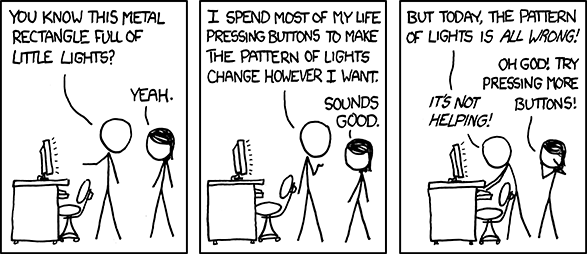
\includegraphics[width=\textwidth]{bilder/computer_lights.png}
}
\end{figure*}

Im Gegensatz zur Schule gibt es an der Uni eine Reihe verschiedenartiger Veranstaltungen, in denen der Lehrstoff vermittelt werden soll. Im wesentlichen sind das: Vorlesungen, Übungen, Seminare und Praktika. Ihr habt im ersten Semester nur mit den ersten beiden zu tun. Diejenigen unter Euch, die Physik studieren, werden ab dem zweiten Semester auch Praktika machen. Proseminare werden in Mathe ab dem zweiten Semester angeboten. Beides braucht Euch also jetzt noch nicht zu beunruhigen. Ihr findet im Verlauf dieses Abschnitts zu beidem noch einiges an Informationen.

\section{Vorlesungen}

Theoretisch sollte in den Vorlesungen eine Dozentin ein abgestecktes Teilgebiet der Mathematik bzw. Physik vermitteln.

Die Praxis sieht jedoch oft anders aus. In der Physik werden in atemberaubenden Tempo erstaunliche Phänomene vorgeführt und zur Erklärung noch erstaunlichere Formeln herangezogen, oft unterstützt durch erstaunlichste Versuche (die mitunter zur Multi-Media-Show geraten).

In Mathe bedecken die Profs in ebenfalls atemberaubendem Tempo gleichmäßig die Tafel mit ebenfalls erstaunlichen Zeichen die, kaum definiert, bereits in abenteuerliche Beweise verwickelt werden. Diese wiederum ermuntern dann einige unterforderte Studis dazu, Quervergleiche zum Lebesgueschen Lemma und ebenfalls verwirrenden Korollaren vorzuschlagen.

Es gibt zwei Wege, um trotz oft unbefriedigender Vorlesungspraxis an Lehrstoff zu kommen, d.h. etwas zu verstehen und nicht gleich am Anfang den Faden zu verlieren. Der eine ist, Fragen zu stellen, auch wenn das häufig Überwindung kostet. Es ist dabei gar nicht so wichtig, ob mit einer Frage etwas sofort klar wird, es ist schon gut, dass durch eine Frage den anderen und sich selbst Gelegenheit gegeben wird, die eigenen Gedanken zu ordnen (und nicht nur mitschreiben zu müssen). Außerdem wird nur so den Dozentinnen gezeigt, dass es überhaupt Fragen gibt und nicht alles selbstverständlich ist. Dabei ist zu sagen, dass man sich mit Fragen nicht unbedingt eine Blöße gibt, denn manche scheinbar „blöde“ Frage hat schon viele Dozentinnen aus dem Konzept geworfen.

Die andere Methode folgt dem Motto: „Gemeinsam macht stark“. Wenn ihr Euch in Arbeitsgruppen zusammensetzt, könnt ihr Vieles klären, was Euch alleine völlig unerklärlich schien. Für das Lösen der Übungsaufgaben (siehe Kapitel „Übungsaufgaben“) ist es sowieso unerlässlich zusammenzuarbeiten, denn nur so könnt ihr damit klar kommen.

\subsection{Formalia}

Ganz richtig ist das mit den verschiedenen Veranstaltungen aber doch nicht. Eigentlich ist nämlich euer gesamtes Studium modularisiert, und jedes Modul eures Studiums eine „zeitlich und thematisch abgeschlossene Lerneinheit“. Ein Modul kann dabei ganz unterschiedlich aufgebaut sein, aber tatsächlich bestehen die meisten Module aus Vorlesung + Übung, Seminar oder Praktikum.

Für ein Modul bekommt ihr dann Leistungspunkte, kurz \gls{LP}. Manchmal liest man auch die Begriffe Credit Points, kurz \gls{CP}, oder gar \gls{ECTS}, kurz ECTS. Diese drei bezeichnen aber immer das gleiche. In eurem Bachelor müsst ihr insgesamt 180 \gls{LP} sammeln, also etwa 30 pro Semester. Ein Leistungspunkt entspricht dabei etwa 30 Stunden Arbeit, wobei das von Modul zu Modul von der Realität mehr oder weniger abweicht.

\subsection{Und wenn ich nicht will?}

Natürlich ist es auch möglich, alle Veranstaltungen (bis auf die Abgabe der scheinpflichtigen Übungsblätter) sausen zu lassen und nur aus Büchern zu lernen. Manchmal, bei sehr schlechten Vorlesungen, ist dies sogar die einzige sinnvolle Möglichkeit etwas zu lernen und seine Zeit sinnvoll zu nutzen. Hier muss jede ihren eigenen Stil entwickeln. Sprecht Euch aber in jedem Fall mit der Übungsleiterin ab, wenn ihr dort regelmäßig fehlen wollt, denn manchmal ist die Anwesenheit und das unfreiwillige Vorrechnen notwendige Voraussetzung für die Scheinvergabe.
